\subsubsection{Electrocardiogram (ECG) data}
\label{subsubsec:results_ecg_1}

After the experiment, the ECG signal processing is organized in the following steps: 

\begin{itemize}
    \item Filtering and removing outliers. Since the participants moved during the whole experience, the sensors also captured some noise data.
    \item Normalization between -1 and 1;
    \item Peak detection and evaluation – if the results were not of good quality, the peak detection method's parameters were adjusted to improve it; 
    \item Calculation of BPM using Kubius HRV Standard;
    \item Calculation of SDNN using Kubius HRV Standard.
\end{itemize}

At the beginning of each experiment, a baseline was collected to establish a comparison between the relaxed state of the participant and the scenes' induced state. However, the results were not consistent.  During the experiment, it was expected that the heart rate would increase compared to the baseline because the participants were at rest. However, for most of the participants, it decreased, indicating a systematic problem may have occurred. Due to this fact, the analysis is based only on absolute values.

\paragraph*{Analysis of the heartbeat frequency (BPM)}\mbox{}\\

Figures \ref{fig:boxplot_ecg_bpm_blind_scene} and \ref{fig:boxplot_ecg_bpm_blind_rounds} brings the corresponding boxplot, grouped by method and round. In both cases, it is not possible to observe significant differences among the methods or rounds.

\begin{figure}[!htb]
    \centering
    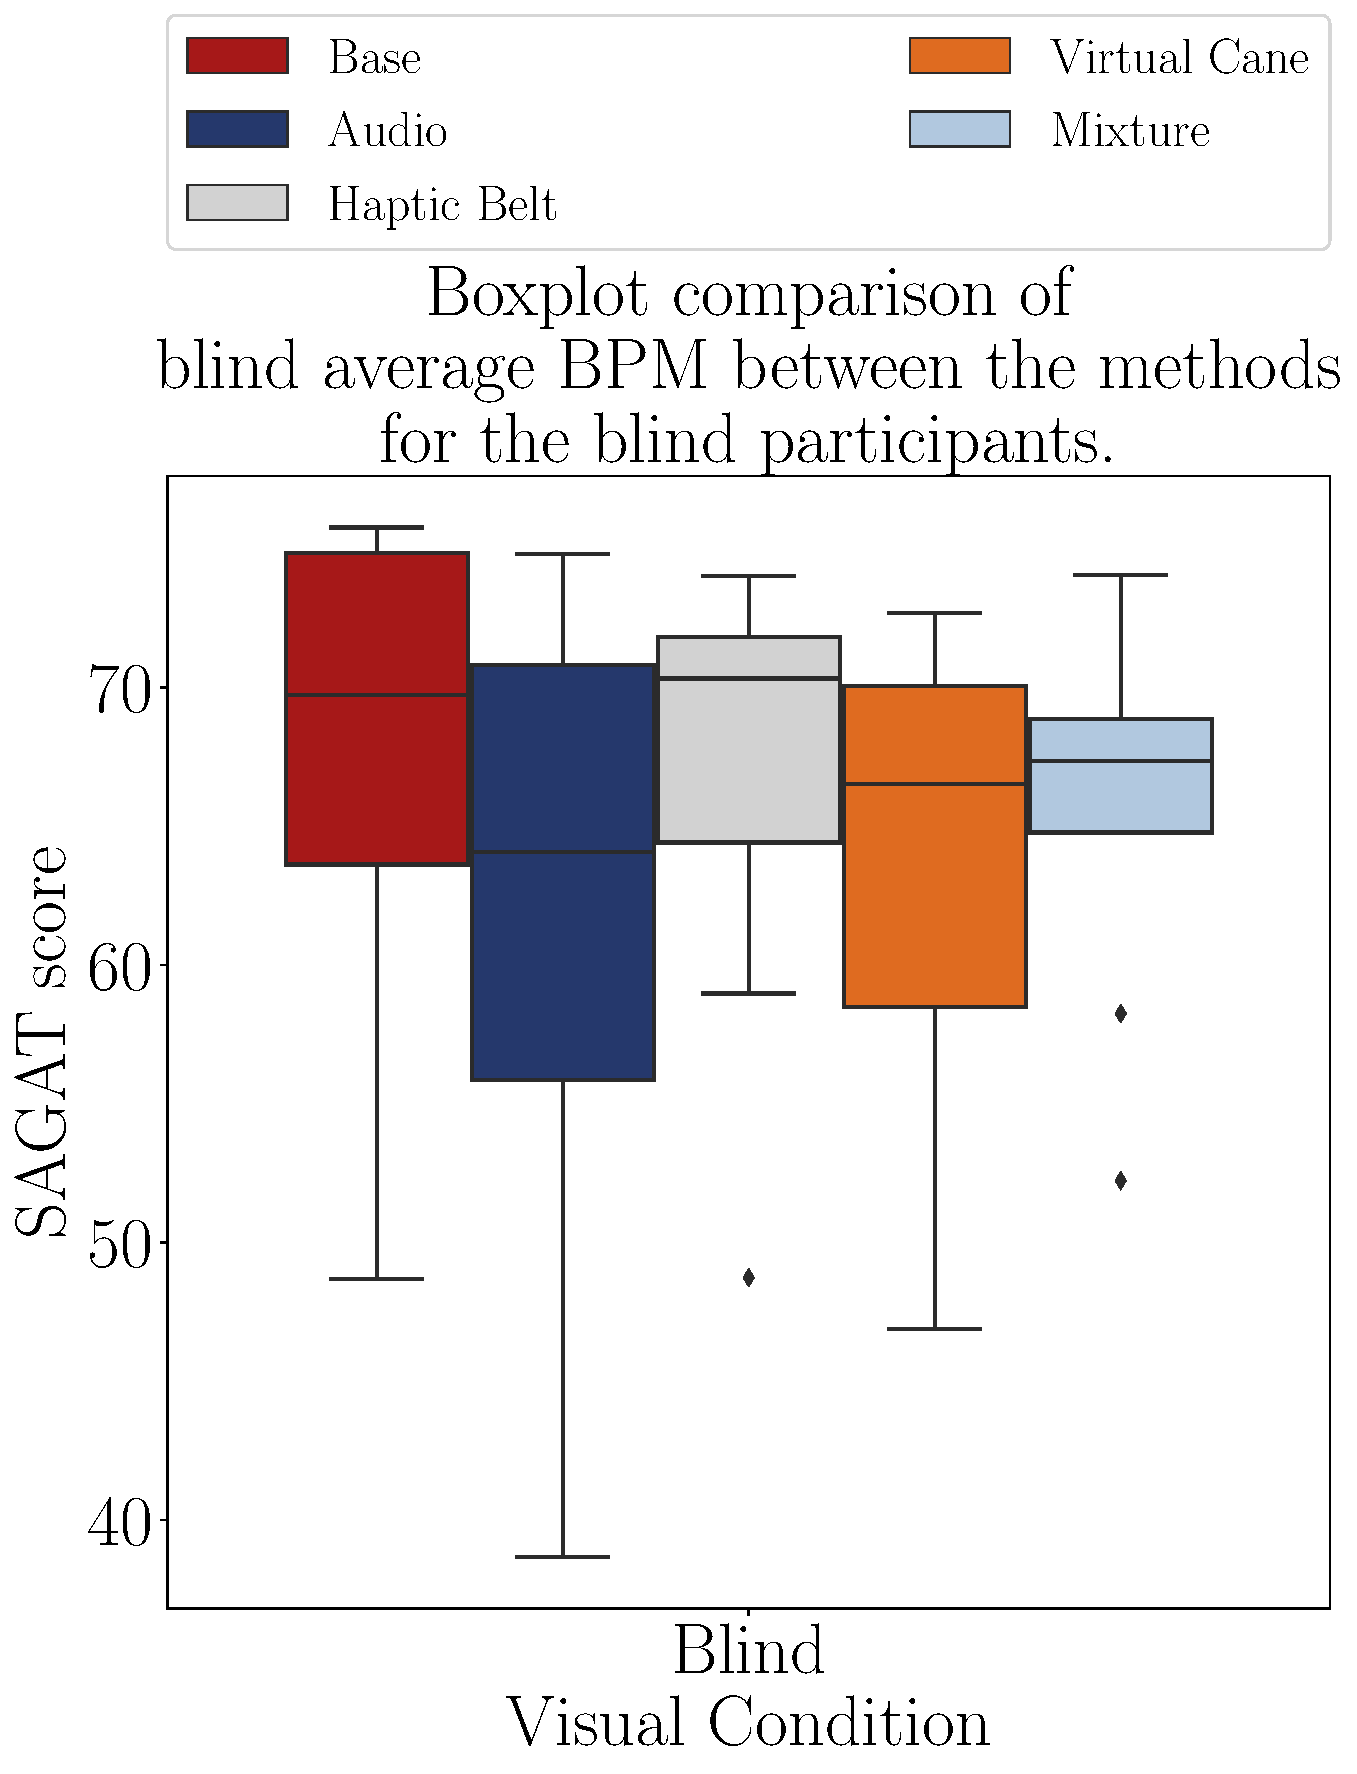
\includegraphics[width = 0.75\linewidth]{3 - Resultados/Figuras/boxplot_ecg_bpm_blind_scene.pdf}
    \caption{Boxplot of the BPM of the blind participants grouped by the methods.}
    \label{fig:boxplot_ecg_bpm_blind_scene}
\end{figure}

\begin{figure}[!htb]
    \centering
    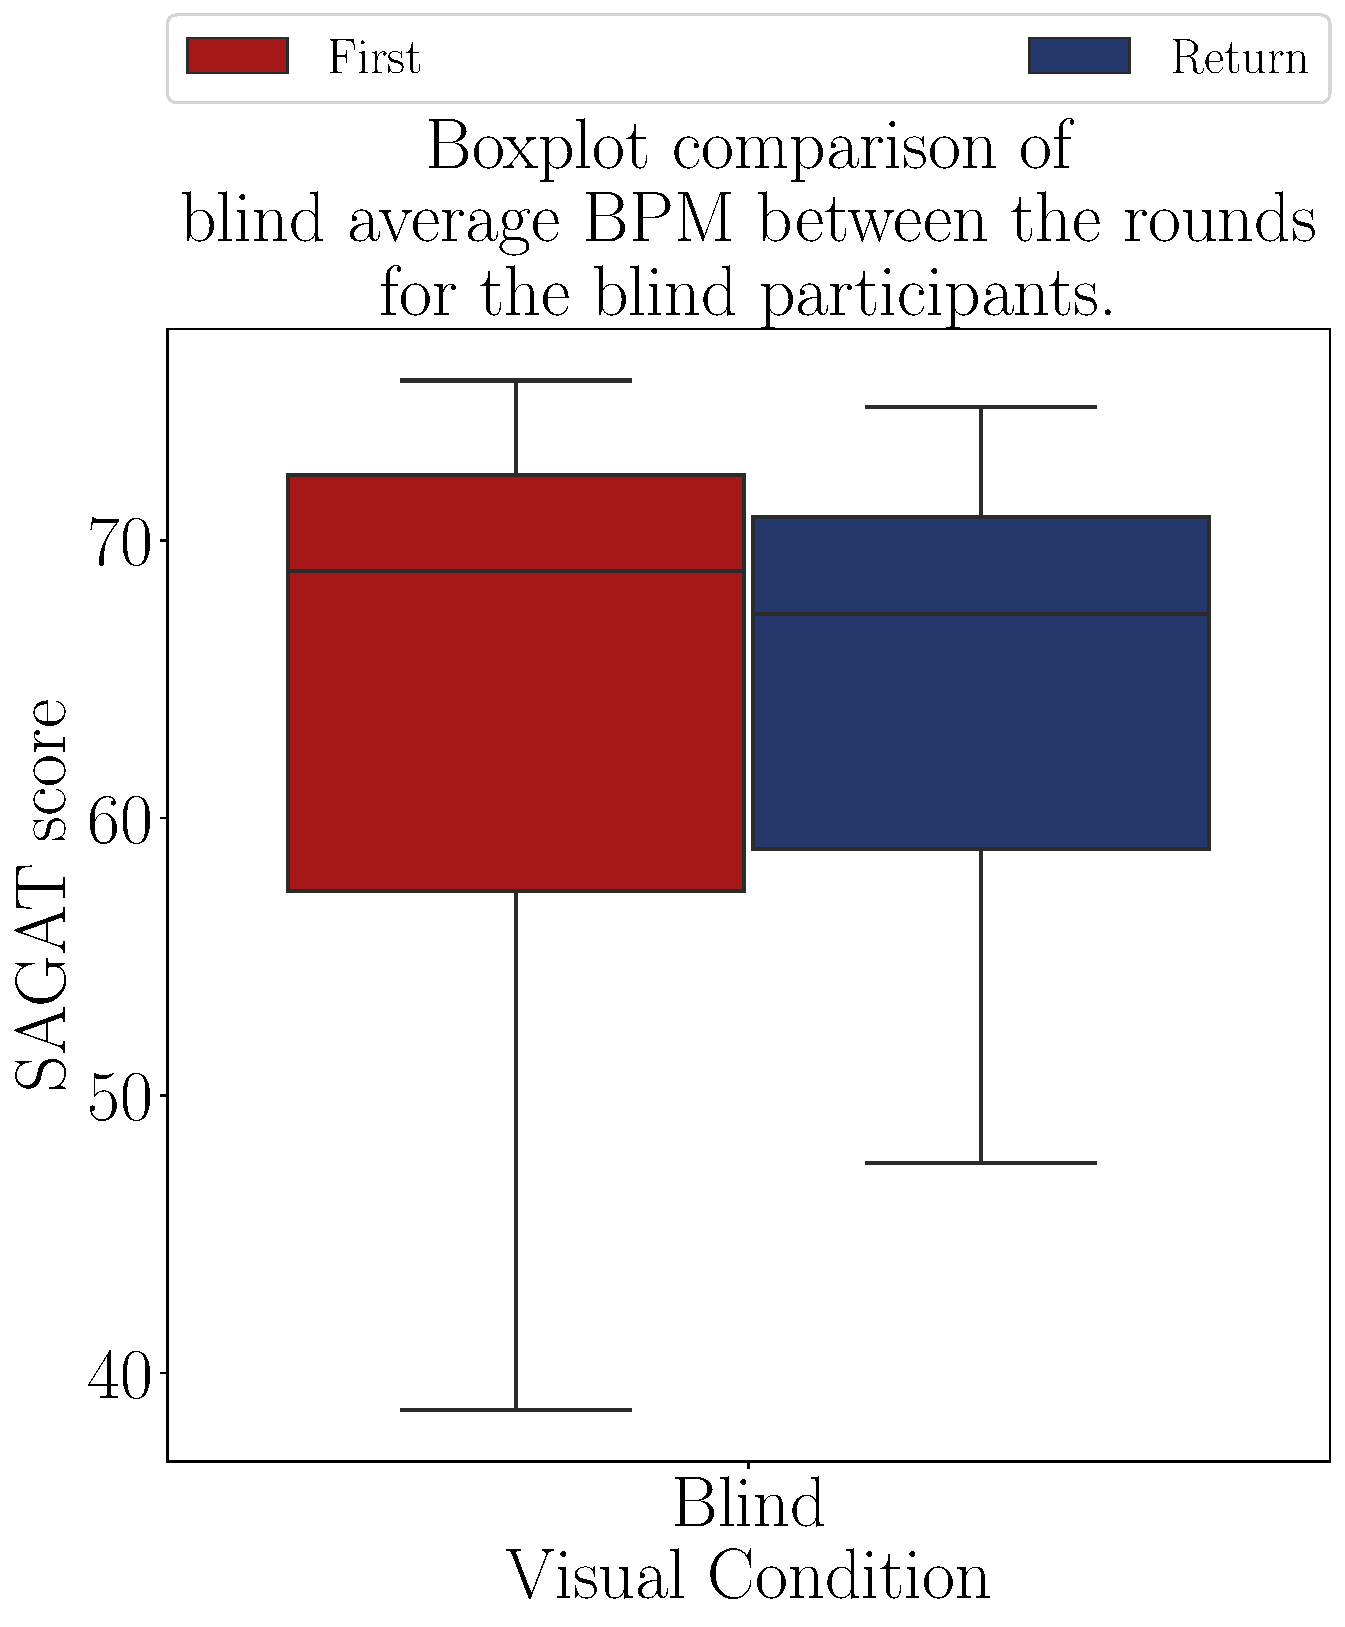
\includegraphics[width = 0.75\linewidth]{3 - Resultados/Figuras/boxplot_ecg_bpm_blind_rounds.pdf}
    \caption{Boxplot of the BPM of the blind participants grouped by the rounds.}
    \label{fig:boxplot_ecg_bpm_blind_rounds}
\end{figure}

The participants do not have a similar variance, which jeopardize the results of ANOVA. Considering this limitation, Table \ref{tab:blocanova_bpm_two_way_blind} brings the p-value obtained by ANOVA, which confirmed the previous analysis, as it does not indicate a significant influence of either the guidance methods or the rounds in the participants' heart rate. 


\begin{table}[!htb]
\centering
\caption{Anova p-value for the BPM -- blinded users.}
\label{tab:blocanova_bpm_two_way_blind}
\begin{tabular}{lrrrrr}
\toprule
          Source & P-Value \\
\midrule
    \    Methods &   0.100 \\
     \    Rounds &   0.371 \\
\    Interaction &   0.894 \\
\bottomrule
\end{tabular}
\end{table}



%%%%%%%%%%%%%%%%%%%%%%%%%%%%%%%%%%%%%%%%%%%%%%%%%%%%%%%%%%%%%%%%%%%%%%%%%%%%
%%%%%%%%%%%%%%%%%%%%%%%%%%%%%%%%%%%%%%%%%%%%%%%%%%%%%%%%%%%%%%%%%%%%%%%%%%%%
%%%%%%%%%%%%%%%%%%%%%%%%%%%%%%%%%%%%%%%%%%%%%%%%%%%%%%%%%%%%%%%%%%%%%%%%%%%%
%%%%%%%%%%%%%%%%%%%%%%%%%%%%%%%%%%%%%%%%%%%%%%%%%%%%%%%%%%%%%%%%%%%%%%%%%%%%

\paragraph*{Analysis of the heartbeat variance (SDNN)}\mbox{}\\

Figure \ref{fig:boxplot_ecg_sdnn_blind_scene} and Figure \ref{fig:boxplot_ecg_sdnn_blind_rounds} bring the SDNN barplot grouped by the methods and the rounds. There is a slight tendency among the participants to increase the heartbeat in the return round.

\begin{figure}[!htb]
    \centering
    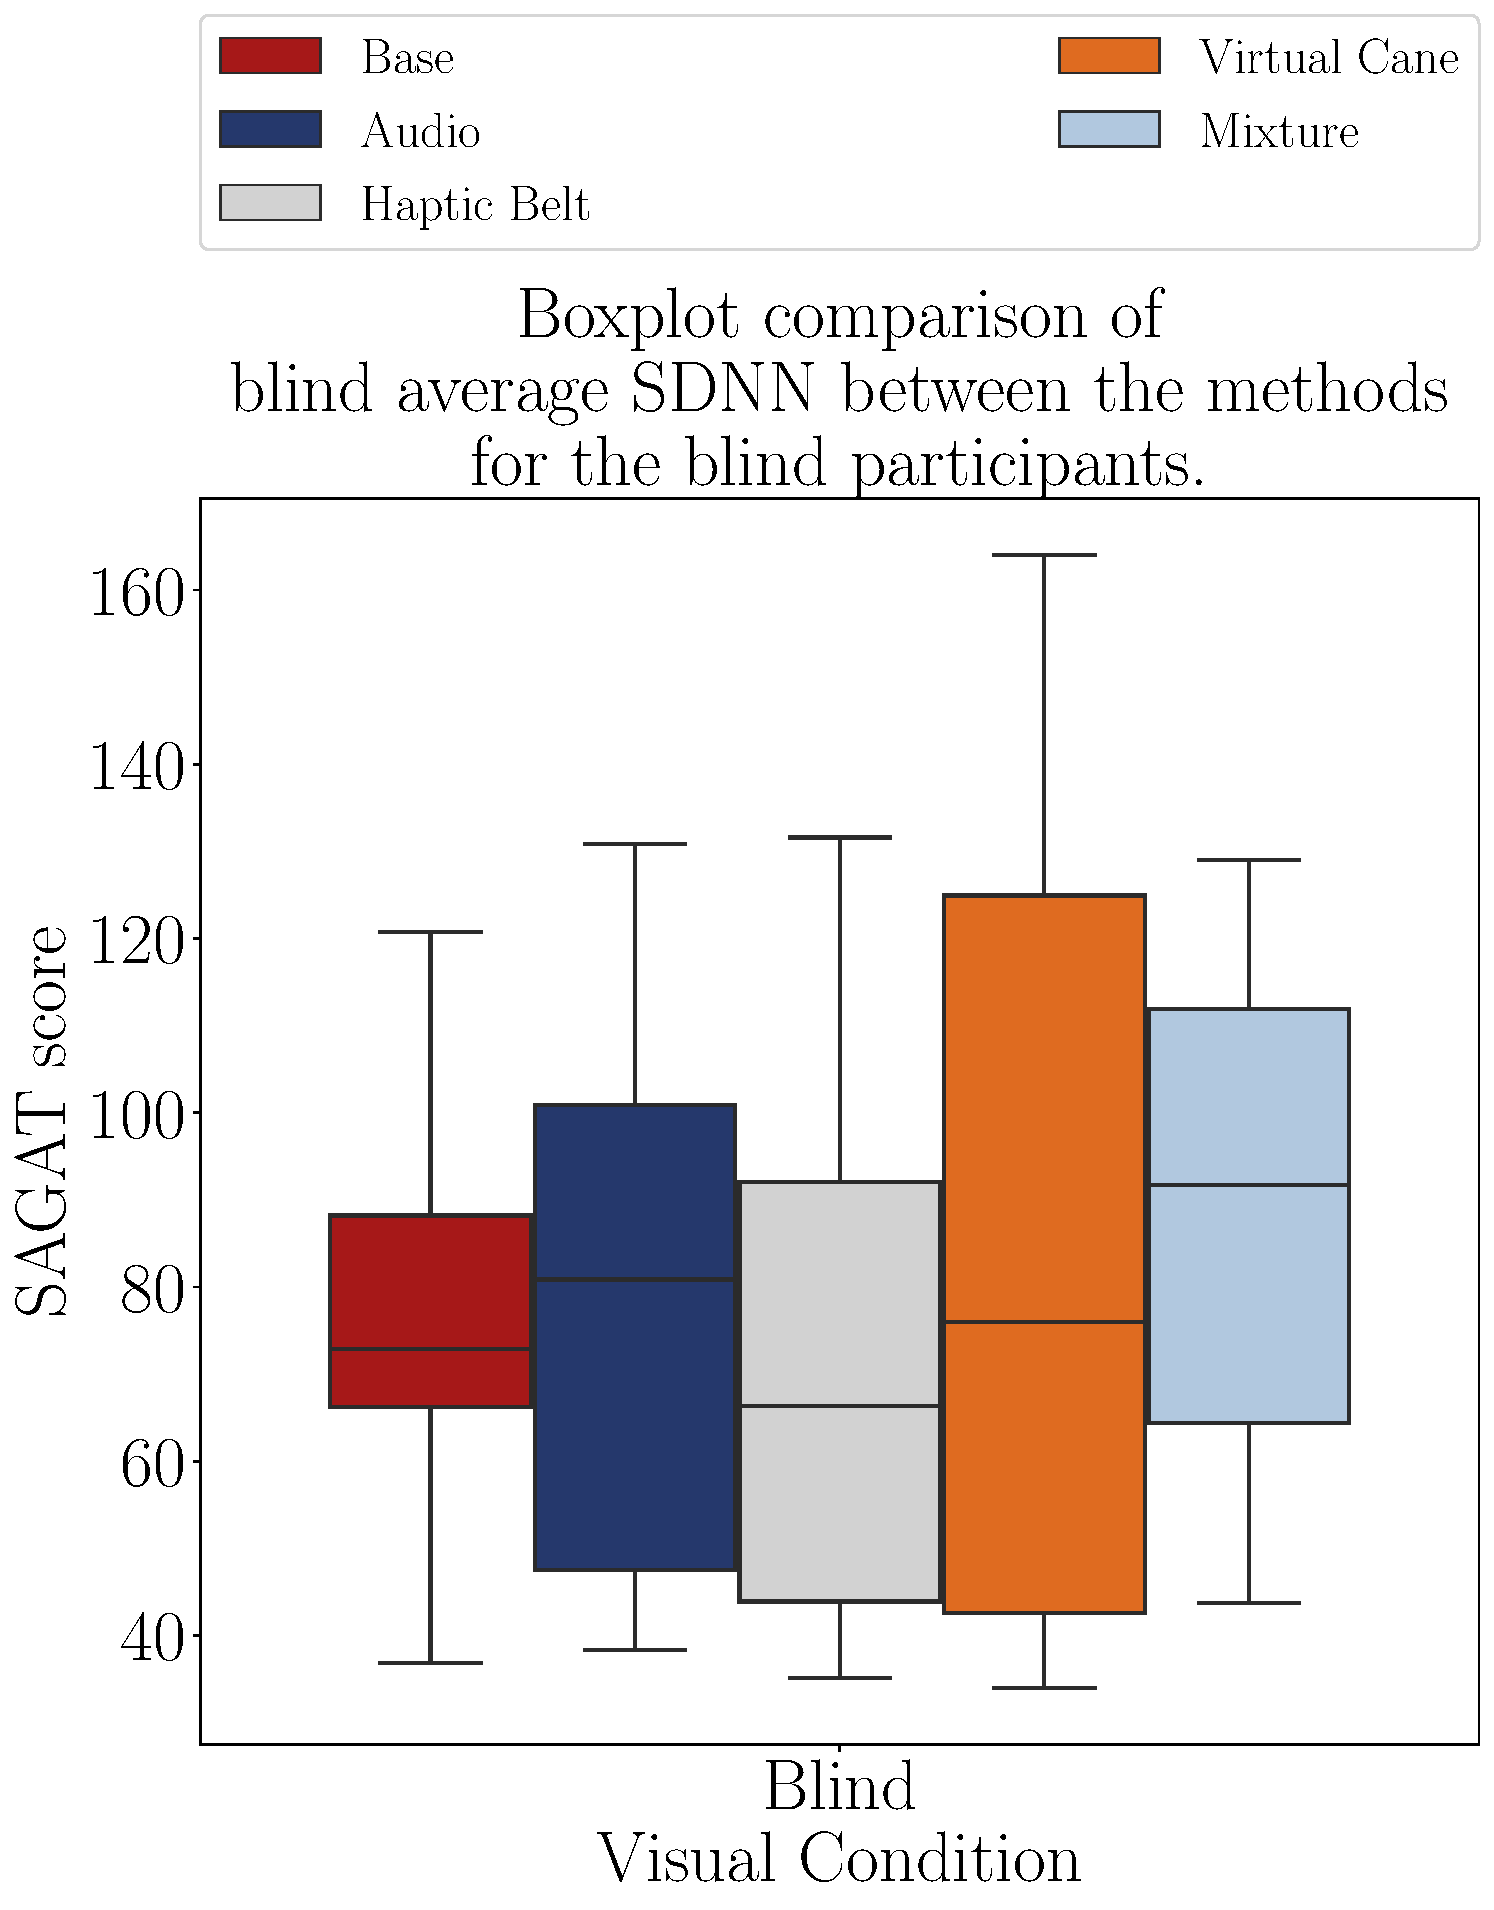
\includegraphics[width = 0.75\linewidth]{3 - Resultados/Figuras/boxplot_ecg_sdnn_blind_scene.pdf}
    \caption{Boxplot of the SDNN of the blind participants grouped by the methods.}
    \label{fig:boxplot_ecg_sdnn_blind_scene}
\end{figure}
\begin{figure}[!htb]
    \centering
    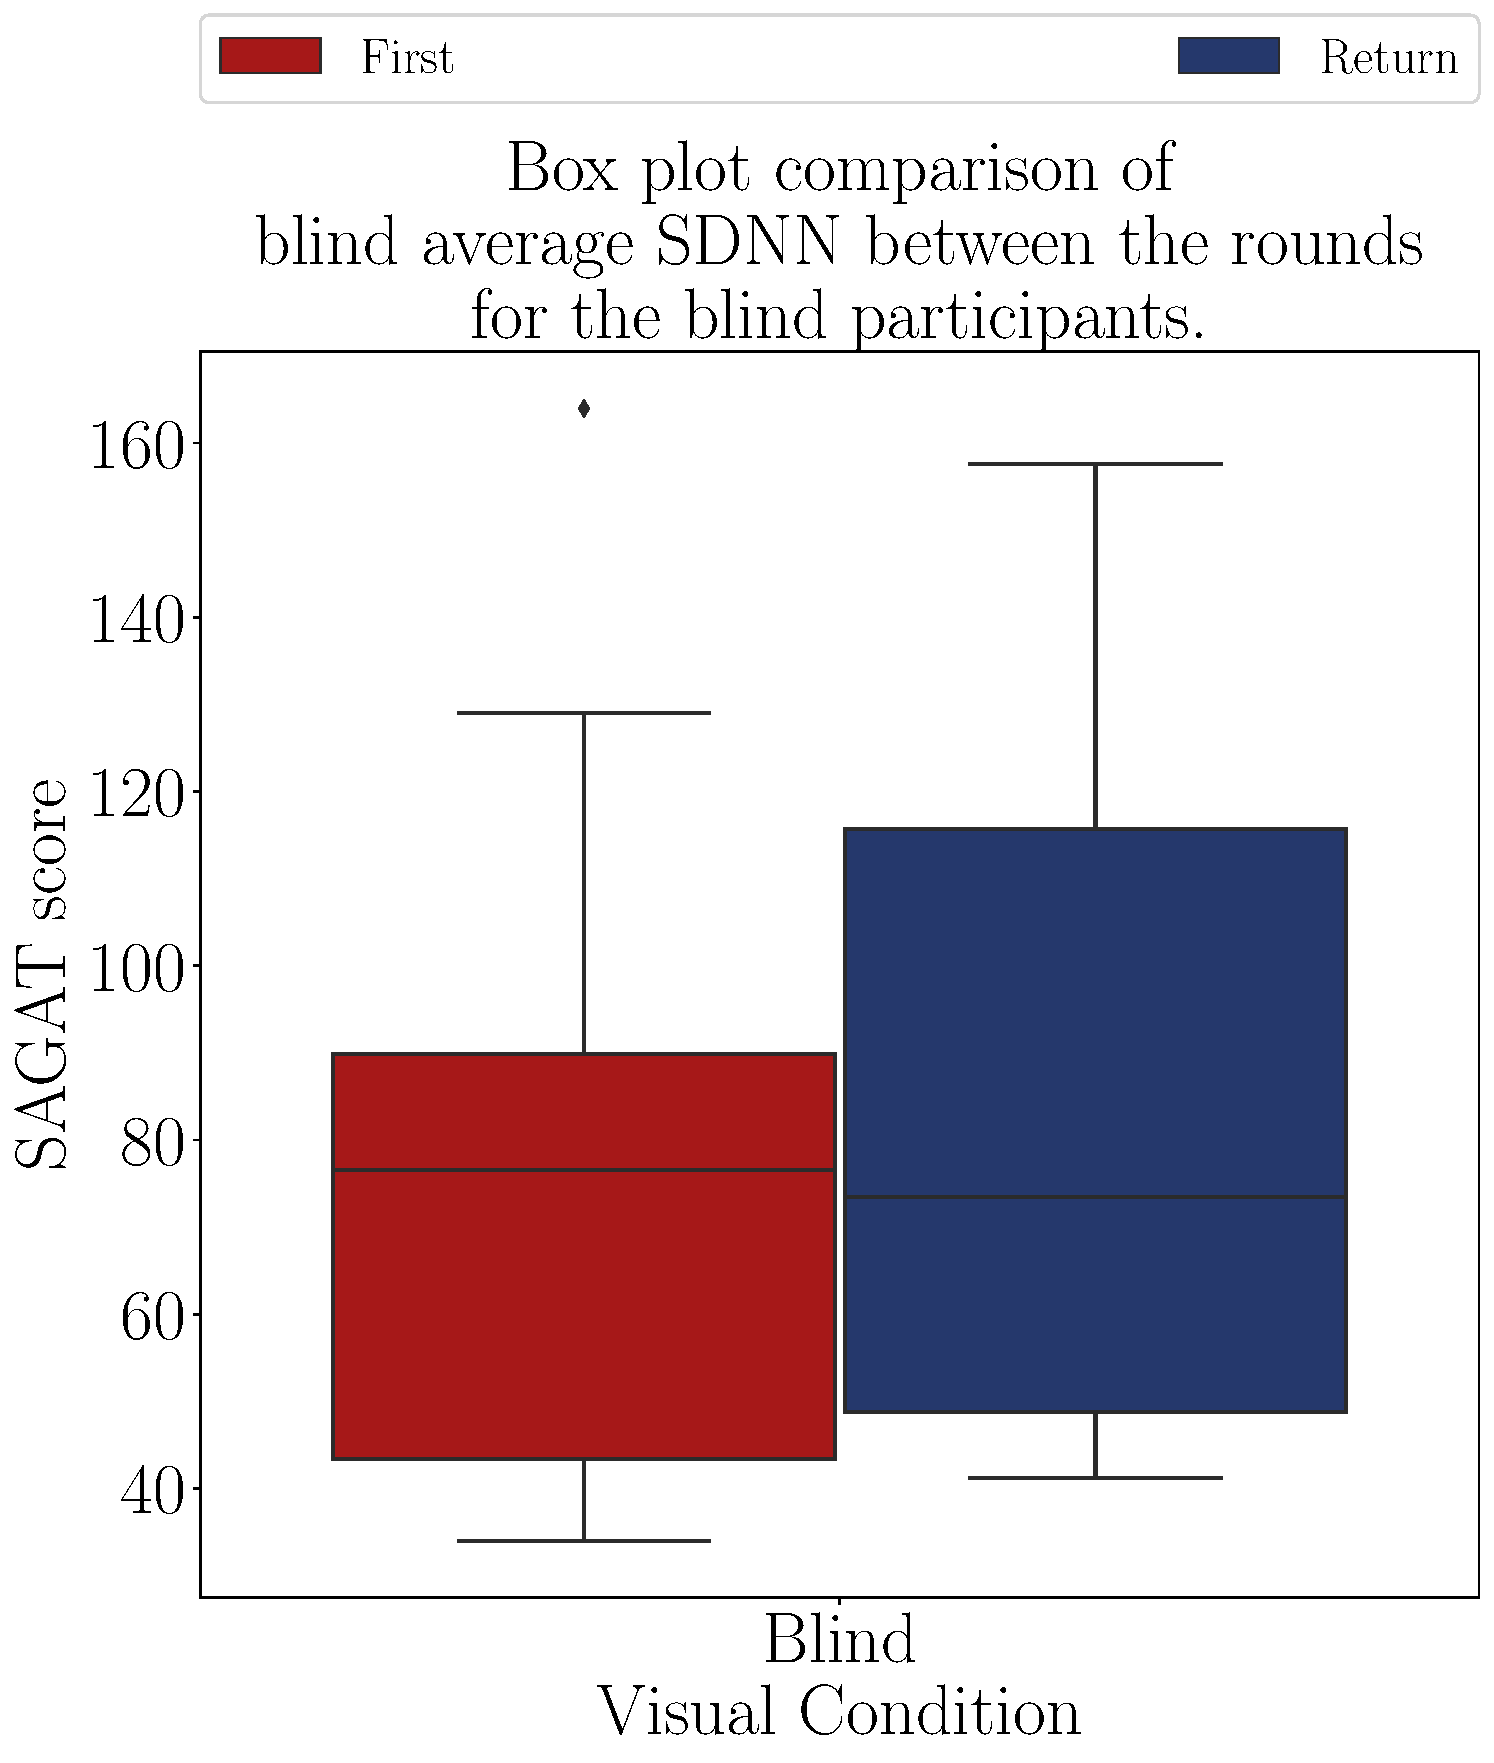
\includegraphics[width = 0.75\linewidth]{3 - Resultados/Figuras/boxplot_ecg_sdnn_blind_rounds.pdf}
    \caption{Boxplot of the SDNN of the blind participants grouped by the rounds.}
    \label{fig:boxplot_ecg_sdnn_blind_rounds}
\end{figure}

The ANOVA results are presented in Table \ref{tab:blocdanova_sdnn_two_way_blind} and do not confirm any influence of the methods nor the rounds on the ECG heart rate variance.


\begin{table}[H]
\centering
\caption{Anova p-value for the average SDNN -- blinded users.}
\label{tab:blocdanova_sdnn_two_way_blind}
\begin{tabular}{lrrrrr}
\toprule
          Source & P-Value \\
\midrule
    \    Methods &   0.486 \\
     \    Rounds &   0.223 \\
\    Interaction &   0.473 \\
\bottomrule
\end{tabular}
\end{table}


